\documentclass[SRC.tex]{subfiles}
\begin{titlepage} % Suppresses displaying the page number on the title page and the subsequent page counts as page 1
	\newcommand{\HRule}{\rule{\linewidth}{0.5mm}} % Defines a new command for horizontal lines, change thickness here
	
	\center % Centre everything on the page
	
	%------------------------------------------------
	%	Headings
	%------------------------------------------------
	
	\textsc{\LARGE HTX Frederikshavn}\\[1.5cm] % Main heading such as the name of your university/college
	
	\textsc{\Large Studieretningscase}\\[0.5cm] % Major heading such as course name
	
	\textsc{\large Matematik og Fysik}\\[0.5cm] % Minor heading such as course title
	
	%------------------------------------------------
	%	Title
	%------------------------------------------------
	
	\HRule\\[0.4cm]
	
	{\huge\bfseries P6 - Studieretningscase}\\[0.4cm] % Title of your document
	
	\HRule\\[1.5cm]
	
	%------------------------------------------------
	%	Author(s)
	%------------------------------------------------
	
	\begin{figure}[h!]
		\centering
		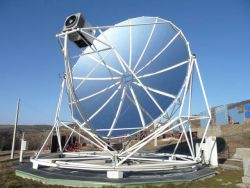
\includegraphics[width=0.4\linewidth]{Billeder/744-9}
		\caption{(promes, u.d.)}
		\label{fig:744-9}
	\end{figure}
	\vfill \vfill
	\begin{minipage}{0.4\textwidth}
		\begin{flushleft}
			\small
			\textit{Af}\\
			\textsc{Christian Kaae Larsen, \\ 2. B} % Your name
		\end{flushleft}
	\end{minipage}
	~
	\begin{minipage}{0.4\textwidth}
		\begin{flushright}
			\small
			\textit{Vejledere}\\
			\textsc{Kasper Weirum Risgaard, \\ Kristian Holm Nielsen} % Supervisor's name
		\end{flushright}
	\end{minipage}
	
	% If you don't want a supervisor, uncomment the two lines below and comment the code above
	%{\large\textit{Author}}\\
	%John \textsc{Smith} % Your name
	
	%------------------------------------------------
	%	Date
	%------------------------------------------------
	
	\vfill\vfill\vfill % Position the date 3/4 down the remaining page
	
	{\large\today} % Date, change the \today to a set date if you want to be precise
	
	%------------------------------------------------
	%	Logo
	%------------------------------------------------
	
	%\vfill\vfill
	%\includegraphics[width=0.2\textwidth]{placeholder.jpg}\\[1cm] % Include a department/university logo - this will require the graphicx package
	
	%----------------------------------------------------------------------------------------
	
	\vfill % Push the date up 1/4 of the remaining page
	
\end{titlepage}
